\begin{figure}[H]
\centering
\begin{minipage}[b]{0.49\textwidth}
\centering
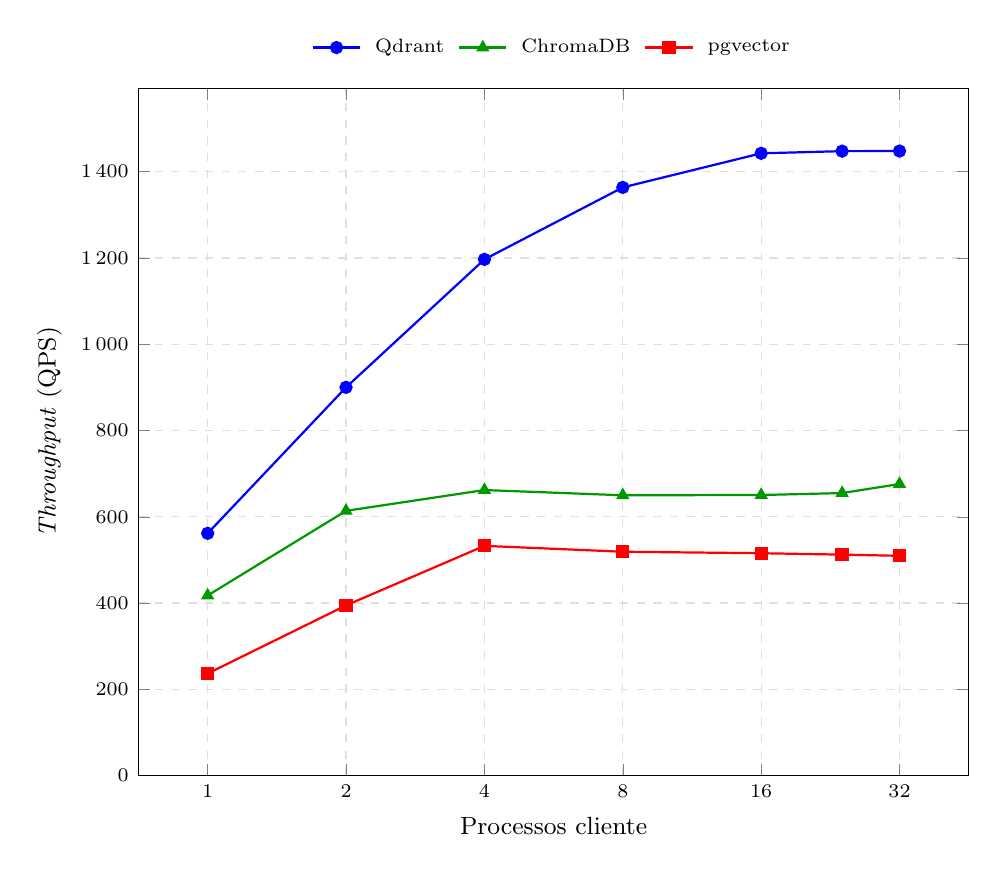
\begin{tikzpicture}
\begin{axis}[
    width=\textwidth, height=0.85\textwidth,
    xlabel={Processos cliente}, ylabel={\textit{Throughput} (QPS)},
    xmode=log, log basis x={2}, xtick={1,2,4,8,16,32}, xticklabels={1,2,4,8,16,32},
    ymin=0,
    /pgf/number format/1000 sep={\,},
    grid=major, grid style={dashed, gray!25},
    legend columns=3, legend style={at={(0.5,1.03)}, anchor=south, font=\scriptsize, draw=none, /tikz/column sep=3pt},
    tick label style={font=\scriptsize}, label style={font=\small}
]
\addplot[color=blue, mark=*, thick] coordinates {(1,561.64) (2,900.06) (4,1196.73) (8,1363.57) (16,1442.60) (24,1447.61) (32,1447.90)};
\addlegendentry{Qdrant}
\addplot[color=green!60!black, mark=triangle*, thick] coordinates {(1,417.55) (2,613.75) (4,662.00) (8,649.82) (16,650.47) (24,654.95) (32,676.00)};
\addlegendentry{ChromaDB}
\addplot[color=red, mark=square*, thick] coordinates {(1,236.57) (2,394.57) (4,532.60) (8,518.95) (16,515.51) (24,512.26) (32,509.49)};
\addlegendentry{pgvector}
\end{axis}
\end{tikzpicture}
\caption*{(a) \textit{Throughput}}
\end{minipage}%
\hfill
\begin{minipage}[b]{0.49\textwidth}
\centering
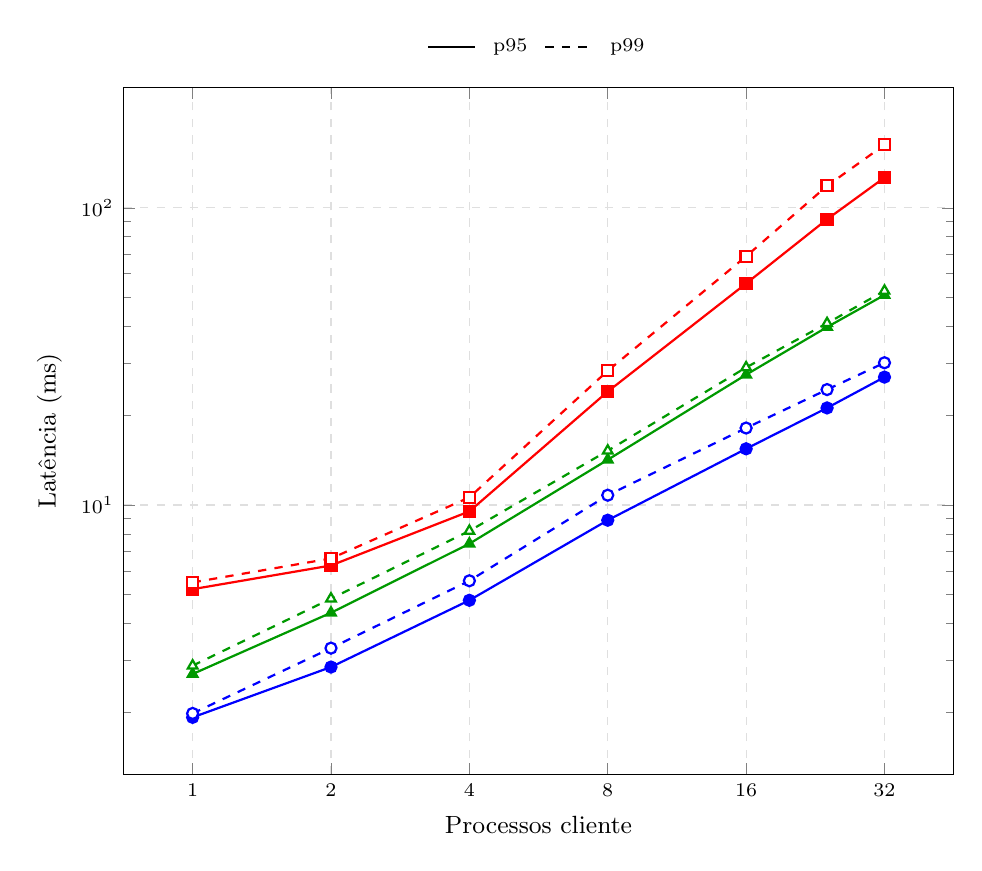
\begin{tikzpicture}
\begin{axis}[
    width=\textwidth, height=0.85\textwidth,
    xlabel={Processos cliente}, ylabel={Latência (ms)},
    xmode=log, log basis x={2}, xtick={1,2,4,8,16,32}, xticklabels={1,2,4,8,16,32},
    ymode=log, log basis y={10},
    /pgf/number format/1000 sep={\,},
    grid=major, grid style={dashed, gray!25},
    legend columns=2, legend style={at={(0.5,1.03)}, anchor=south, font=\scriptsize, draw=none, /tikz/column sep=4pt},
    tick label style={font=\scriptsize}, label style={font=\small}
]
\addplot[color=blue, mark=*, thick, forget plot] coordinates {(1,1.93) (2,2.85) (4,4.78) (8,8.89) (16,15.46) (24,21.22) (32,26.94)};
\addplot[color=blue, mark=*, mark options={solid, fill=white}, thick, dashed, forget plot] coordinates {(1,1.99) (2,3.30) (4,5.56) (8,10.79) (16,18.16) (24,24.46) (32,30.11)};
\addplot[color=green!60!black, mark=triangle*, thick, forget plot] coordinates {(1,2.70) (2,4.34) (4,7.41) (8,14.20) (16,27.45) (24,39.70) (32,50.89)};
\addplot[color=green!60!black, mark=triangle*, mark options={solid, fill=white}, thick, dashed, forget plot] coordinates {(1,2.88) (2,4.84) (4,8.18) (8,15.23) (16,29.03) (24,40.88) (32,52.56)};
\addplot[color=red, mark=square*, thick, forget plot] coordinates {(1,5.21) (2,6.26) (4,9.52) (8,24.09) (16,55.63) (24,91.51) (32,126.41)};
\addplot[color=red, mark=square*, mark options={solid, fill=white}, thick, dashed, forget plot] coordinates {(1,5.49) (2,6.61) (4,10.61) (8,28.30) (16,68.68) (24,118.56) (32,162.90)};
\addlegendimage{black, thick}\addlegendentry{p95}
\addlegendimage{black, thick, dashed}\addlegendentry{p99}
\end{axis}
\end{tikzpicture}
\caption*{(b) Latências p95 e p99}
\end{minipage}
\caption{\textit{Throughput} e latências p95 e p99 sob concorrência crescente para a \textbf{Métrica L2} (mediana de 3 réplicas). No painel (b), cada motor mantém a cor do painel (a); a linha contínua corresponde ao p95 e a tracejada ao p99, em escala logarítmica.}
\label{fig:throughput_concorrencia_l2}
\end{figure}
